\section{Literature review}

My research is located at the intersection of three main subjects:
\begin{itemize}
	\item \st{music technology and} Interactive music\st{al} systems \new{for non-professional musicians}\st{ (including mobile)},
	\item \new{modern, technology dependent, social phenomena}
	\item \new{and social effects of music} \st{social interaction, and location based services.}
\end{itemize}
\st{In this review I will shortly describe each subject}\new{I will start this review with a brief introduction to interactive music systems, followed by a short description of each of the above subjects}, elucidating only the aspects relevant to my research\st{, while exploring some of the recent studies showing possible connections between these subjects}. \new{I will end this review by presenting how those different fields combines together, and stand on the importance of each one of them to my work.}

\subsection{A brief introduction to interactive music systems}

% \new{According to the Oxford Dictionary to ``interact'' is to ``act in such a way as to have an effect on each other'' (}\todo{add ref}\new{). ``Act'' and ``affect'' are visibly the main concepts of interactivity. In the field of interactive music systems these ideas may be implemented in different ways, \st{. It could be playing a music instrument (ref), interacting with an installation (Visnjic, 2010), distribute the control over the music to different people (DistributedDJ) and more. Interactive music systems}} ranging from \new{interactive sound installations, where participants interact with physical objects around them to affect the sound} \st{very basic types of controllers that use some physical input to generate music} (Visnjic, 2010\st{; Silver, 2011; Flanagan, 2009}, \href{http://createdigitalmusic.com/2012/10/at-musicmakers-experiencing-music-through-design-as-community-of-doers-collaborates-listen-watch/}{\todo{finish another ref}}) to much complex approaches \new{that, as manifested by MIT Opera of the Future research group,} aim\new{s}\st{ing} to ``explore concepts and techniques to help advance the future of musical composition, performance, learning, and expression'' (\href{http://www.media.mit.edu/research/groups/opera-future}{``Opera of the future''})\st{; Palmer, 2009.)}.

According to the Oxford Dictionary to ``interact'' is to ``act in such a way as to have an effect on each other'' (\todo{add ref}). ``Act'' and ``affect'' are visibly the main concepts of interactivity. In the field of interactive music systems these ideas may be implemented in different ways, ranging from new instrument designs to collaborations with robotic performers (Eigenfeldt and Kapur 2008).\todo{find a way to add the quote by ``opera of the future'' here}

Since the beginning of the exploration \new{in the field} of \new{interactive} music \st{interactive} system\new{s} in the nineteen-sixties, different researchers and composers created systems that were able to interact with performer in a live situation. First examples of this kind of \st{interactive music are} \new{interactive systems} \new{were} Gordon Mumma's Hornpipe, and Morton Subotnick's Touch\new{, where specially designed electronic systems alter the input from the performer in some nondeterministic, yet musically defined, manner} (\href{http://blog.lib.umn.edu/geers001/emusic/14_assig_ComposingInteractiveMusicCh1-2.pdf}{Winkler, 2001: 12}).

Later, programming languages designed for musical applications began to be developed, such as GROOVE by Max Mathews and Richard Moore at Bell labs (Mathews and Moore, 1970). \new{Using those languages musicians was able to create system like those of Mumma and Subotnick programmatically}\todo{change reference to MUSIC-1 and rewrite last sentence, can also use Koenig project 1}.

In the nineteen-eighties, a group of musical instruments manufacturers agreed on standard method for sending and receiving musical information digitally, establishing \new{the }MIDI \new{protocol} as a universal standard (\href{http://www.insidetechnology360.com/index.php/the-history-of-midi-8862/}{Quinn, 2010}). The standardization of sending and receiving information combined with the emergence of personal computers enabled the creation of \st{commercial and open source} \new{modern} programing languages for musical application\new{s}\st{, the most important one today is}. Max/MSP (\href{http://cycling74.com/whatismax/}{\st{``What is Max?''}}) \new{which began its development} by Miller Puckette \st{from IRCAM, Paris} in 1986 \new{may be a good example} (\href{http://blog.lib.umn.edu/geers001/emusic/14_assig_ComposingInteractiveMusicCh1-2.pdf}{Winkler, 2001: 16}). \new{As opposed to early programming languages as GROOVE, most of those personal computer based languages not only still exist today but also keep progressing and new music oriented programing languages are written every year} (\todo{ref ChucK or Usine Hollyhock}).\st{ One of the main uses of these new programming languages was to compose interactive music that can manipulate sound during performance in real-time.}

\new{But the proliferation of the personal computer not only drive the creation of programing languages for music application. In the nineteen-nineties} \st{Due to new opportunities in digital signal processing technologies in the nineteen-nineties, and the proliferation of personal computers,} digital audio workstations (DAW) became a common alternative to analog recording \new{equipment} \st{systems} in \st{recording} studios (\todo{find reference}). Later, with the arrival of the VST standard (\href{http://www.steinberg.net/en/company/technologies.html}{``Steinberg technologies''}) \st{and Ableton Live (}\href{https://www.ableton.com/en/live/}{\st{``What is Live?''}}), computers became \new{even more essential tool for music production.} \st{the main tool for audio manipulation in real time.} \new{Those changes also find their way to the stage with the emergence of live performance oriented DAWs as Ableton Live (}\href{https://www.ableton.com/en/live/}{\new{``What is Live?''}}\new{) and software based DJ setups in late nineteen-nineties.}

\new{Another key event in the history of interactive music systems is the appearance of the Arduino platform in 2006. The Arduino is an easy to use hardware and software package, ``intended for artists, designers, hobbyists and anyone interested in creating interactive objects or environments.'' (}\todo{Arduino homepage ref here}\new{) Until its appearance the only way for a musician to interact with music creation software was through audio and MIDI. But from then }\st{When microcontrollers like the Arduino platform (``Arduino'') began to appear in mid 2000's} a lot of new ways of controlling audio started to be possible, mostly by translating physical properties of the space into sound.

\subsection{Interactive music systems for non-professional musicians}

In addition to systems that interact with a performer or professional musician there are also interactive music systems for non-professional musicians. In the following paragraphs I will show some different approaches to this concept.

% interactive video clips: Interlude, Chris Milk and Aaron Koblin
In the last years an interactive type of video clips start to emerge. Those video clips share some of the elements traditionally kept for the director to viewers. As a relatively new phenomena video clips like those are rare but dominant. As examples one can find the works of Chris Milk and Aaron Koblin (\todo{ref}) and the startup Interlude which driven by equivalent concept (\todo{ref}).

% mobile applications: Smule and RjDj
The emergence of modern mobile phones with their high computation power led developers to develop new mobile applications for music creation for non-professional musicians. Those applications gives the average user the ability to create music by himself and without musical education. Good examples for this kind of applications Smule's applications , with emphasis on AutoRap (\todo{ref}). On the other hand, the same technology open the opportunity to consume interactive music or rather ambient sonification that affected by the user surrounding as demonstrated by RjDj (\todo{ref to video demonstration}).

% interactive sound installations: objects with sound, project ADA
Sound installations are installations located in the three dimensional space that dialog with their surroundings through sound (\href{http://en.wikipedia.org/wiki/Sound_installation}{``Sound installation''}). Sound installations are not always interactive, i.e. they may not response to participants or viewers actions, this kind of installations are irrelevant for this research. Whereas in some interactive installations the main interaction is between the viewer and the installation itself (Visnjic, 2010) there are installations that aims to engage the participants to interact with one another (\todo{ref SPECS project ADA}). One may say that the main goal of this kind of interaction is to facilitate social interaction\todo{find ref, maybe Omer Golan}.

% social DJing: DistributedDJ, the BLOB and playmysong
Furthermore, recent projects suggest to share the role of the DJ in a bar or party between the participants (\todo{ref DistributedDJ}). Using those systems participants can choose the music by themselves and the ``playlist'' is created dynamically by the musical taste of the participants. Most of those project are implemented as mobile applications and some them even integrate social elements in their projects (\todo{ref the BLOB and playmysong}).

% summarize the interactivity trend
Although the above researches and projects are only a small portion of the work that has been done in the field of interactive music systems for non-professional musicians it clearly demonstrates how new technology could be used to allow the average user to participate both in interactive music creation and consumption, as well as in the social interactions they may create.

\subsection{Modern, technology dependent, social phenomena}

% Silent disco and flash mobs. LBS are out because they are not really relevant!

The fast growth of social media produced modern types of social behavior. When the modern mobile devices replaced the old mobile communication devices they became more than just a communication tool (Srivastava, 2005). Two particular phenomena that emerged from that situation that are relevant to my study are silent disco, and flash mobs.

Silent disco \st{/ rave are different names for the same} \new{is the} phenomenon of partying where the music is heard through headphones instead of loudspeakers. The origins of the phenomena is unclear, but it began to be an ordinary way of partying toward the beginning of 2000's (\href{http://en.wikipedia.org/wiki/Silent_disco}{``Silent disco''}). The new phenomena already changed the possibilities of an ordinary party. One new possibility was having two DJs spin two completely different sets side by side at the same party where each participant has two channel wireless headphones, and can decide which DJ to listen to (\href{http://headphonedisco.com/about.php}{``About headphone disco''}). Needless to say, this is not possible with a regular loudspeaker setup.

Another phenomenon relevant to my research is that of flash mobs: \st{``A public gathering of strangers and acquaintances organized via email and texting. Once gathered, flash mobbers perform a quirky stunt and then quickly disperse. This social act shone briefly and brilliantly in cities around the world in summer 2003 and is believed to represent a significant moment in the history of mobile communication'' (Nicholson, 2005).} \new{``A group of people who assemble suddenly in a public place, perform an unusual and seemingly pointless act for a brief time, then quickly disperse, often for the purposes of entertainment, satire, and artistic expression. Flash mobs are organized via telecommunications, social media, or viral emails''} (\href{http://en.wikipedia.org/wiki/Flash_mob}{``Flash mob''}). \new{With regards to the definition above, with emphasis on the way flash mobs are organized and executed, different researchers see the flash mobs as a significant event in the history of mobile communication (Nicholson, 2005).} \st{Flash mobs today make use of new technology to enable distributed parties when the music is determined by the flash mob participants in real time (``Decentralized Dance Party'')}\todo{seems that it's more relevant to silent disco}. \st{Recent studies proposed that a potential for artistic intent and social critique inherently exists in the flash mob's appropriation of the city as a scenographic, performative space (Brejzek, 2010)}. \new{On the other hand, a recent study by Brejzek suggests that a potential for artistic intent inherently exists in the flash mob phenomenon (2010).}

\st{From the different fields of study related to music technology, the most important area for my research is that relating to music interaction systems and audio based augmented reality systems.}

\st{Today, most social networks combine LBS in their platform. Examples are Foursquare, Facebook and their purchase of Gowalla (Laughlin, 2011), Google plus ``Check in'' and more. Recent studies of this service market also show the growth of the usage of LBS among users (Zickuhr and Smith, 2011; Miltsch, 2010), and of mobile users who don't use mobile LBS, 60\% are willing to consider using it (Lawrence, 2012).}

\subsection{Social effects of music}

% Based, as suggested by Avi, on ``The social psychology of music -- David Hargreaves''.

\subsection{Roadmap}\label{roadmap}

% Describe the system and its connection with concepts mentioned before. Everything bellow is new!

The system developed in this research has been inspired by the concepts of interactive music systems and intended for the average user. It sees both silent disco and flash mobs as significant conceptional roots. Whereas silent disco will be referred as a context for the system existent, flash mobs are associated as a social phenomena that use new technologies to facilitate creative, or even artistic social behavior.

From the participants point of view the system will consist of few balloon bundles, each one corresponds to a specific musical styles. When the participants will stroll between the balloon bundles with their mobile devices and headphones their relative distances from the different bundles will affect the music in their headphones. In addition, participants will be able to freely move the balloon bundles, thereby changing the structure of the music in the virtual space.

\begin{figure}[h]
	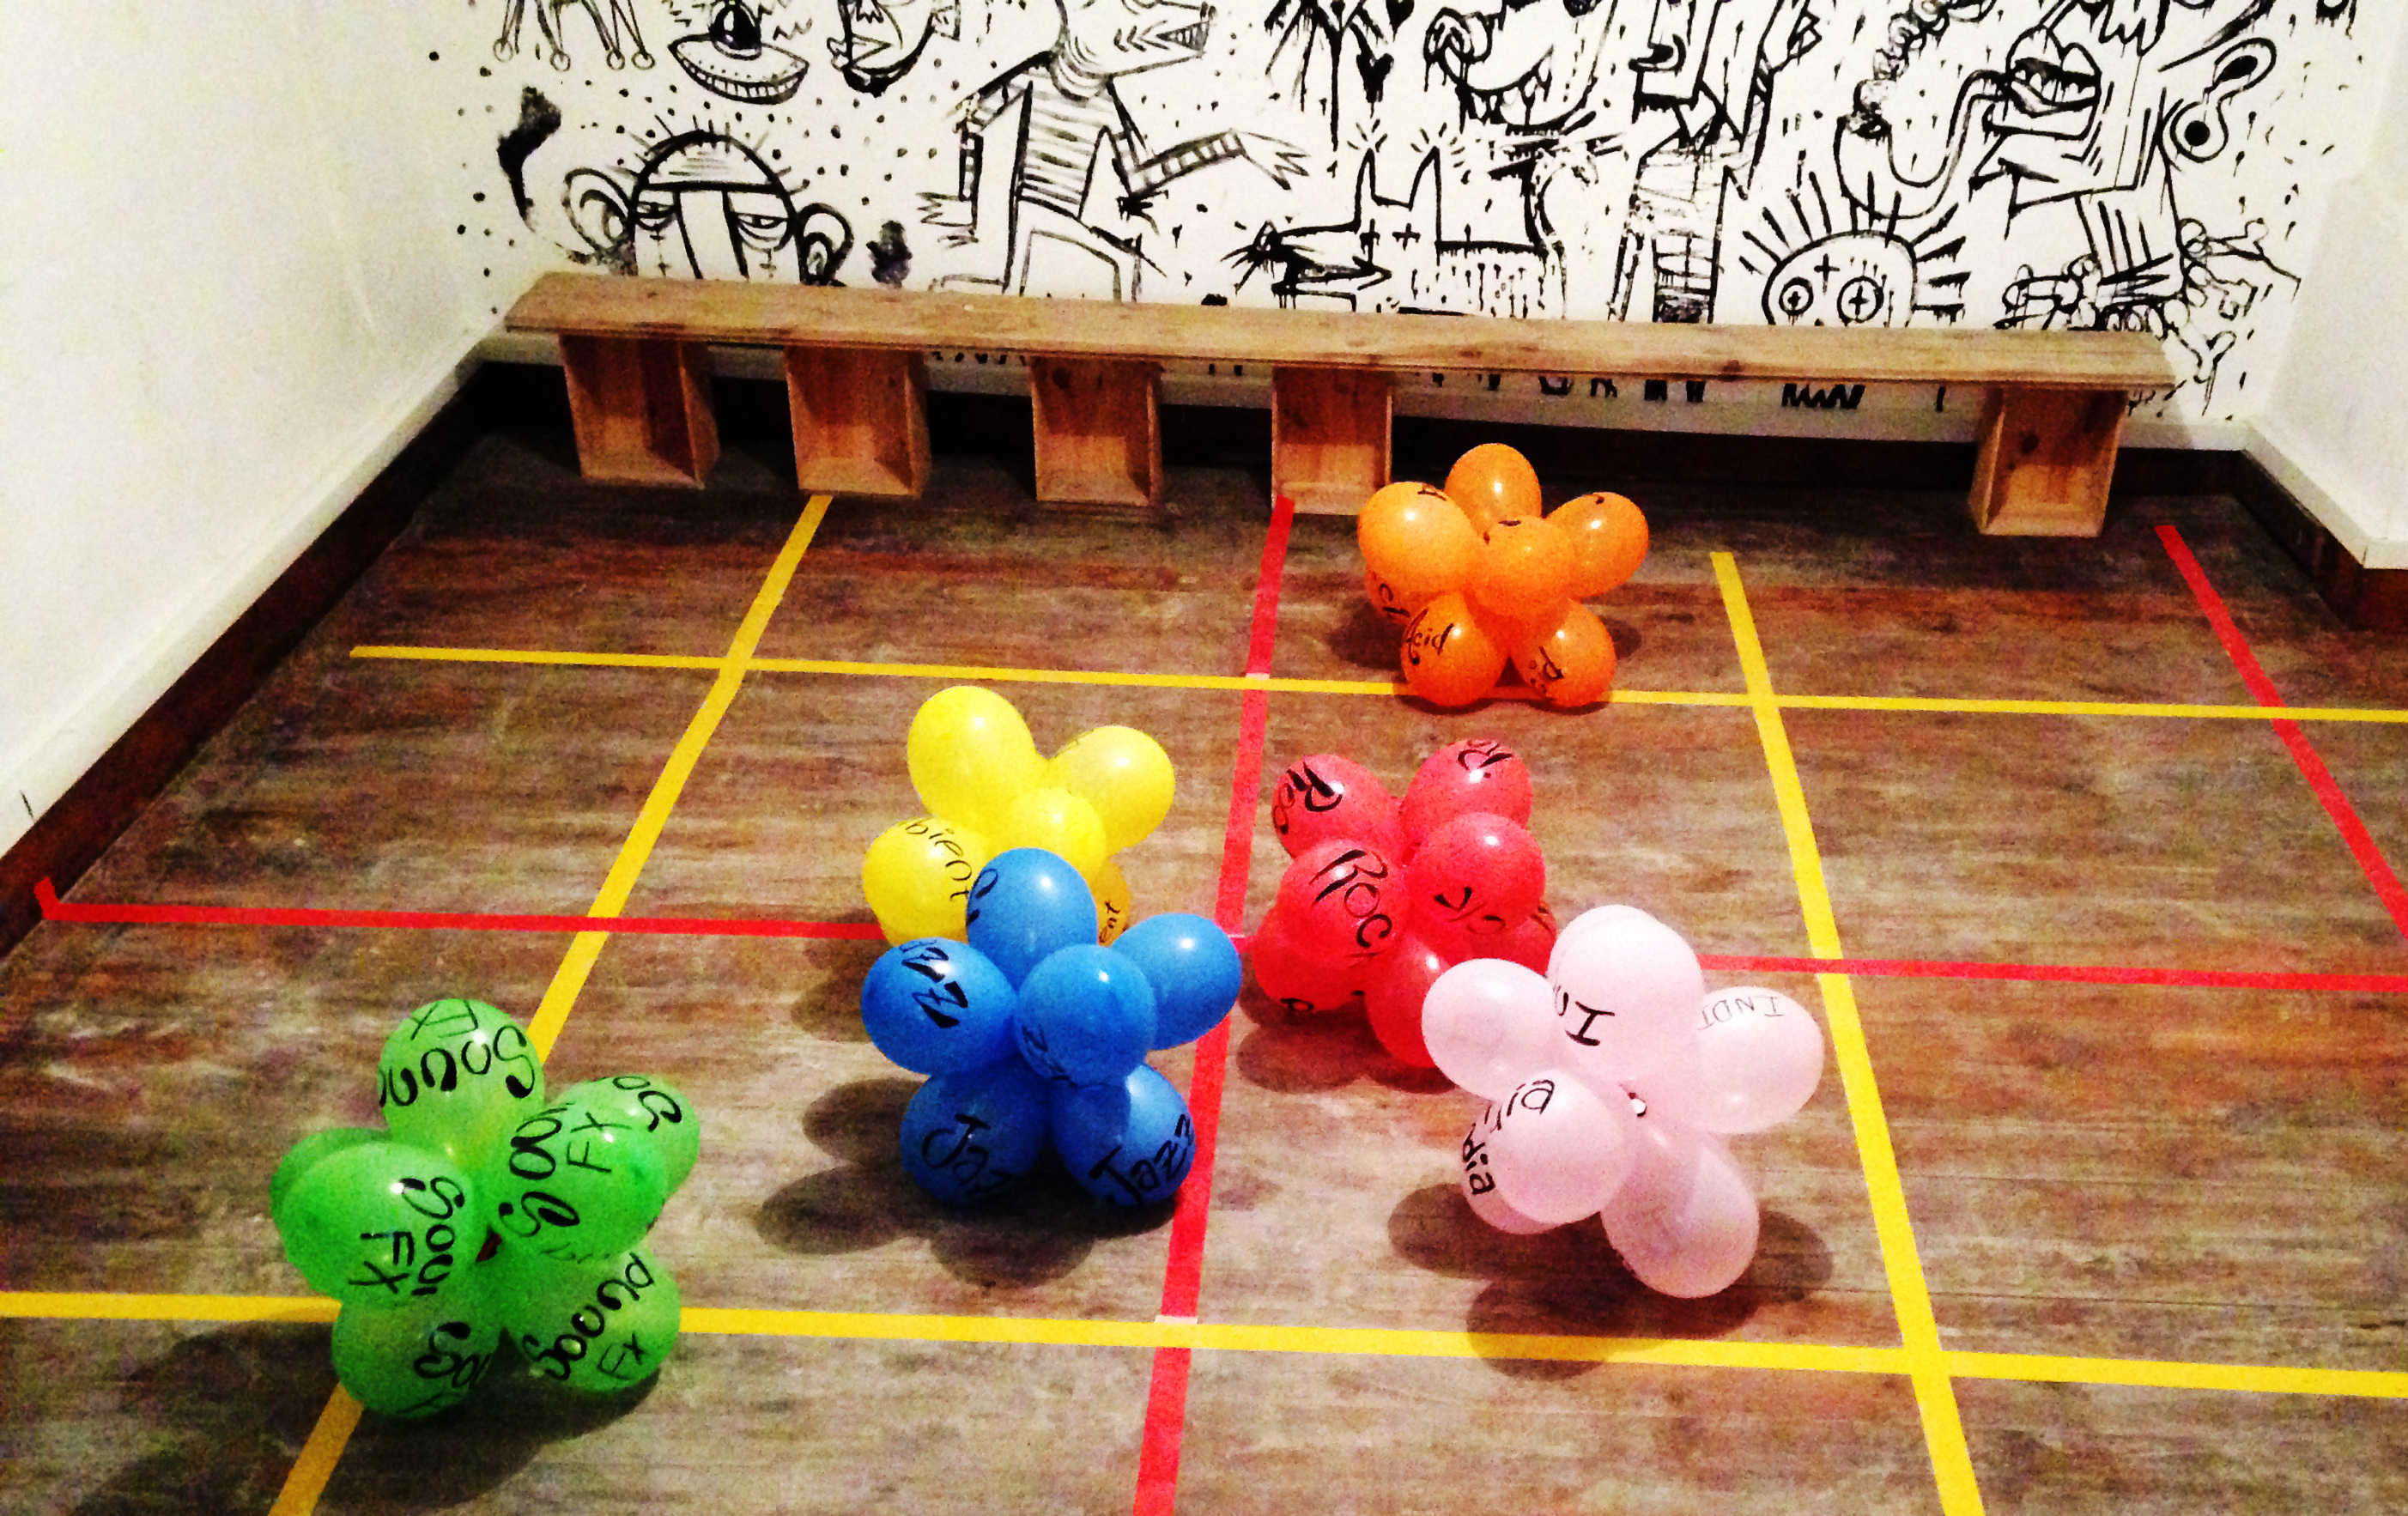
\includegraphics[width=\linewidth]{balloons}
	\caption{Balloon bundles on the dance floor}
\end{figure}

Finally, in order to evaluate the social effect of this system I will try to answer the research question: \emph{Does the system elaborate social interaction between participants in an interactive silent disco party?}